\documentclass[11pt]{article}
\usepackage[margin=1in]{geometry}
\usepackage{booktabs}
\usepackage{amsmath}
\usepackage{tikz}
\usetikzlibrary{positioning,arrows.meta}
\usepackage{hyperref}
\usepackage{enumitem}
\usepackage{float}
\setlist{nosep}

\title{Pentium M Style Hybrid Branch Predictor\\\large COSC6385 Computer Architecture --- Branch Predictor Assignment}
\author{ChengAo Shen \\ \small Student ID: 2437132}
\date{October 2026 \\ \small Code: \url{https://github.com/ChengAoShen/cosc6385-branch-predictor}}

\begin{document}
\maketitle

\section{Summary}

I implemented the direction predictor of the Pentium M (\texttt{pm\_predictor} in
\texttt{src/my\_predictor.h}) on the CBP-2 infrastructure. It combines a bimodal
table with a tagged, 4-way set-associative global predictor. A hit in the global
table overrides the bimodal prediction.

\begin{table}[H]
\centering
\begin{tabular}{lrr}
\toprule
Predictor & Storage & Average MPKI (20 traces) \\
\midrule
Always taken (original \texttt{pm\_predictor}) & 0 & 86.312 \\
Sample gshare (32K entries, 15-bit history) & 8 KB & 6.306 \\
\textbf{This design} & \textbf{4.75 KB} & \textbf{5.495} \\
\bottomrule
\end{tabular}
\end{table}

The final design has 12.9\% fewer mispredictions than gshare with about 60\% of
its storage, and it is better than gshare on 18 of 20 traces.

Not implemented (allowed by the assignment): the loop predictor, target
prediction, and the PIR hash. The global index uses
\texttt{address XOR history} instead of the PIR.

\section{Design}

\begin{figure}[H]
\centering
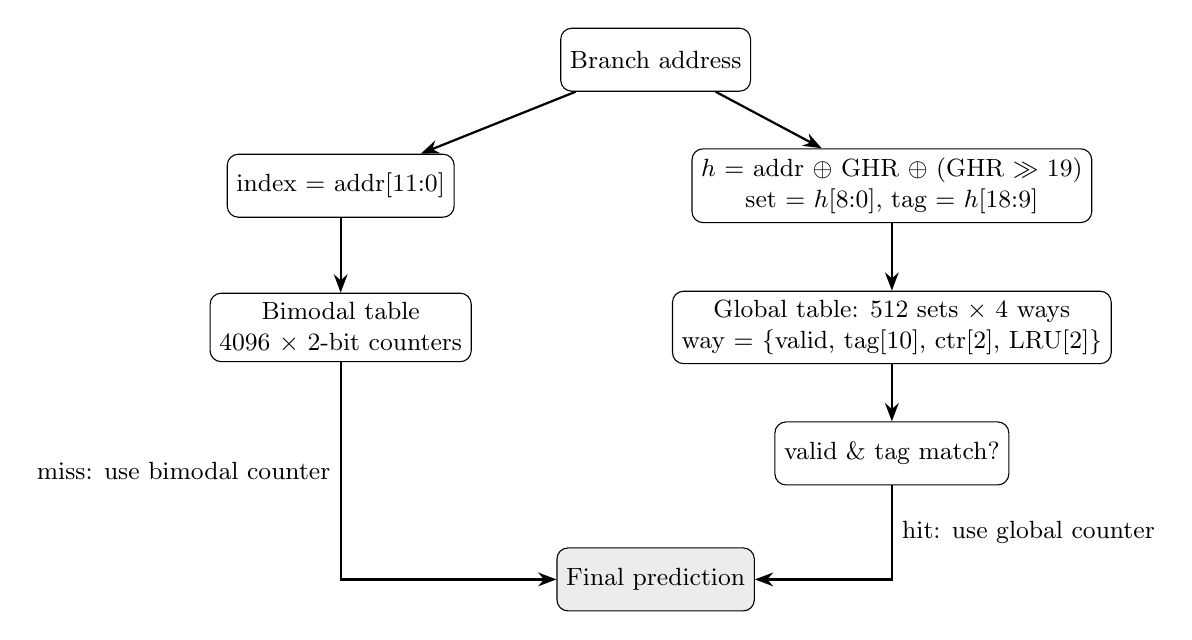
\begin{tikzpicture}[
  box/.style={draw, rounded corners, align=center, minimum height=8mm, font=\small},
  arr/.style={-{Stealth}, thick}]
\node[box] (pc) at (0,0) {Branch address};
\node[box] (bidx) at (-4,-1.6) {index = addr[11:0]};
\node[box] (hash) at (3,-1.6) {$h$ = addr $\oplus$ GHR $\oplus$ (GHR $\gg$ 19)\\set = $h$[8:0], tag = $h$[18:9]};
\node[box] (bim) at (-4,-3.4) {Bimodal table\\4096 $\times$ 2-bit counters};
\node[box] (glob) at (3,-3.4) {Global table: 512 sets $\times$ 4 ways\\way = \{valid, tag[10], ctr[2], LRU[2]\}};
\node[box] (hit) at (3,-5.0) {valid \& tag match?};
\node[box, fill=gray!15] (mux) at (0,-6.6) {Final prediction};
\draw[arr] (pc) -- (bidx);
\draw[arr] (pc) -- (hash);
\draw[arr] (bidx) -- (bim);
\draw[arr] (hash) -- (glob);
\draw[arr] (glob) -- (hit);
\draw[arr] (hit) |- node[pos=0.25, right, font=\small] {hit: use global counter} (mux);
\draw[arr] (bim) |- node[pos=0.25, left, font=\small] {miss: use bimodal counter} (mux);
\end{tikzpicture}
\caption{Structure of the predictor.}
\end{figure}

\subsection{Tables and storage}

\begin{table}[H]
\centering
\begin{tabular}{llr}
\toprule
Structure & Size & Bits \\
\midrule
Bimodal table & 4096 $\times$ 2-bit counters & 8{,}192 \\
Global table & 512 sets $\times$ 4 ways $\times$ (1 valid + 10 tag + 2 counter + 2 LRU) & 30{,}720 \\
Global history register & 21 bits & 21 \\
\midrule
\textbf{Total} & & \textbf{38{,}933 ($\approx$ 4.75 KB)} \\
\bottomrule
\end{tabular}
\end{table}

The table sizes (4K bimodal entries, 2K global entries, 4 ways) follow the
Pentium M structure described by Milenkovi\'c et al.~\cite{pm}.

\subsection{Index and tag}

\begin{itemize}
\item Bimodal index: \texttt{addr \& 0xFFF} (low 12 bits of the branch address).
\item Global hash: $h = \text{addr} \oplus \text{GHR} \oplus (\text{GHR} \gg 19)$;
      set $= h[8{:}0]$ (512 sets), tag $= h[18{:}9]$ (10 bits).
\item Set and tag together use 19 bits. The GHR has 21 bits, so the
      $\text{GHR} \gg 19$ term folds the two oldest history bits back into the
      hash. Without folding, history bits above bit 18 have no effect.
\end{itemize}

\subsection{Prediction}

\begin{enumerate}
\item If the branch is not conditional, predict taken (as in the original code).
\item Compute the bimodal index, the global set and the global tag, and save them
      in \texttt{pm\_update} for the update step.
\item Search the 4 ways of the set for an entry with \texttt{valid = 1} and a
      matching tag.
\item Hit: direction = MSB of the global counter. Miss: direction = MSB of the
      bimodal counter.
\end{enumerate}

\subsection{Update (conditional branches only)}

\begin{enumerate}
\item Bimodal counter: always updated (2-bit saturating, 0--3).
\item Global hit: update the counter of the hit way and make that way MRU.
\item Global miss: if the bimodal prediction was wrong, allocate the LRU way
      (valid = 1, write the tag, counter = \texttt{taken ? 2 : 1}, make it MRU).
      If bimodal was correct, do not allocate (Pentium M policy).
\item $\text{GHR} \leftarrow ((\text{GHR} \ll 1) \,|\, \text{taken}) \bmod 2^{21}$.
\end{enumerate}

Non-conditional branches do not change counters or the GHR, because only
conditional-branch direction misses are counted. LRU uses a 2-bit age per way
(0 = most recently used); the victim is the way with age 3. Initially all
bimodal counters are 1 (weakly not taken) and all global entries are invalid.

\section{Results}

MPKI = mispredictions per 1000 instructions (lower is better).

\begin{table}[H]
\centering
\small
\begin{tabular}{lrrr}
\toprule
Trace & Always taken & gshare & This design \\
\midrule
164.gzip & 70.025 & 12.473 & 12.574 \\
175.vpr & 85.312 & 13.415 & \textbf{12.900} \\
176.gcc & 86.071 & 11.254 & \textbf{8.279} \\
181.mcf & 102.497 & 15.837 & 16.560 \\
186.crafty & 48.651 & 5.837 & \textbf{5.190} \\
197.parser & 78.421 & 10.008 & \textbf{8.259} \\
201.compress & 76.983 & 7.831 & \textbf{7.366} \\
202.jess & 92.343 & 1.562 & \textbf{0.910} \\
205.raytrace & 109.506 & 2.756 & \textbf{1.861} \\
209.db & 91.451 & 3.909 & \textbf{3.354} \\
213.javac & 109.644 & 2.267 & \textbf{2.029} \\
222.mpegaudio & 110.339 & 2.188 & \textbf{2.013} \\
227.mtrt & 112.022 & 2.657 & \textbf{1.957} \\
228.jack & 77.958 & 3.033 & \textbf{1.808} \\
252.eon & 24.226 & 1.807 & \textbf{1.273} \\
253.perlbmk & 66.833 & 2.554 & \textbf{1.329} \\
254.gap & 75.950 & 3.926 & \textbf{2.538} \\
255.vortex & 70.524 & 1.222 & \textbf{0.706} \\
256.bzip2 & 178.257 & 0.094 & \textbf{0.056} \\
300.twolf & 59.221 & 21.489 & \textbf{18.939} \\
\midrule
\textbf{Average} & 86.312 & 6.306 & \textbf{5.495} \\
\bottomrule
\end{tabular}
\caption{Per-trace MPKI. Bold = better than gshare.}
\end{table}

gzip and mcf are slightly worse than gshare. These traces have many
data-dependent branches, and gshare's 32K counters suffer less from capacity
pressure.

\section{Parameter Study}

The starting point is the configuration suggested in the homework guide: 4K
bimodal, 512 sets $\times$ 4 ways, 6-bit tag, 15-bit history, no folding,
allocation only on a bimodal miss (5.954). One parameter is changed at a time
unless noted.

\begin{table}[H]
\centering
\small
\begin{tabular}{lrl}
\toprule
Change & Avg.\ MPKI & Note \\
\midrule
Baseline & 5.954 & \\
Allocate on every global miss & 6.700 & pollutes the table with easy branches \\
2 ways / 8 ways & 6.466 / 5.767 & \\
256 / 1024 / 2048 sets & 6.348 / 5.689 / 5.527 & 2048 sets = 4$\times$ global storage \\
Tag 4 / 8 / 10 bits & 6.786 / 5.803 / 5.766 & short tags give false hits \\
Bimodal 1K / 16K & 6.206 / 5.872 & \\
History 8 / 12 bits & 7.317 / 6.450 & too little history \\
History 18 / 24 bits (no folding) & 5.954 / 5.954 & extra bits never reach the hash \\
Tag 8, history 18 / 21, folded & 5.603 / 5.563 & \\
Tag 10, history 15 / 18, folded & 5.766 / 5.707 & \\
\textbf{Tag 10, history 21, folded (final)} & \textbf{5.495} & \\
2048 sets $\times$ 8 ways, 16K bimodal & 4.914 & $\approx$33 KB, 7$\times$ storage \\
\bottomrule
\end{tabular}
\end{table}

\noindent Findings:
\begin{enumerate}
\item \textbf{Allocation policy matters most.} Allocating only when the bimodal
      predictor is wrong keeps easy branches out of the global table. Always
      allocating costs about +0.75 MPKI.
\item \textbf{Tag width controls aliasing.} A 4-bit tag causes false hits;
      10 bits is enough.
\item \textbf{History helps only if it reaches the hash.} With set + tag = 15
      bits, a longer history had no effect until the extra bits were folded in.
\item \textbf{Bigger tables help with diminishing returns.} I kept the Pentium M
      sizes instead of the 33 KB configuration.
\end{enumerate}

\section{How to Reproduce}

\begin{verbatim}
make -C src
./run.sh traces          # prints per-trace MPKI and the average
\end{verbatim}

\noindent \texttt{run.sh} is a bash version of the original \texttt{run} script
(which needs \texttt{csh} and \texttt{dc}). Each parameter is a macro
(\texttt{PM\_BIM\_BITS}, \texttt{PM\_SET\_BITS}, \texttt{PM\_WAYS},
\texttt{PM\_TAG\_BITS}, \texttt{PM\_HIST\_LEN}, \texttt{PM\_FOLD},
\texttt{PM\_ALLOC}) and can be set with \texttt{-D} at compile time.

\begin{thebibliography}{9}
\bibitem{pm} M.~Milenkovi\'c, A.~Milenkovi\'c, and J.~Kulick,
  ``Demystifying Intel Branch Predictors,'' Workshop on Duplicating,
  Deconstructing, and Debunking (WDDD), 2002.
\bibitem{cbp} The 2nd JILP Championship Branch Prediction Competition (CBP-2)
  simulation infrastructure and traces.
\bibitem{mcf} S.~McFarling, ``Combining Branch Predictors,'' WRL Technical Note
  TN-36, 1993.
\bibitem{slides} COSC6385 lecture slides, Lecture 6 \& 7: Branch Prediction.
\end{thebibliography}

\end{document}
